\documentclass{amsart}

% For revision control
\usepackage{rcs-multi}
\rcsid{$Id$}
\rcsid{$Header$}
\rcskwsave{$Author$}
\rcskwsave{$Date$} 
\rcskwsave{$Revision$}
%%\rcsRegisterAuthor{devangel}{Dennis Jos{\'e} Evangelista}
\rcsRegisterAuthor{devangel}{Dennis J. Evangelista}

\usepackage{graphicx}
\usepackage[usenames,dvipsnames]{color}
%\usepackage{makeidx} % incompatible with ams art
\usepackage{siunitx}
\DeclareMathOperator*{\argmin}{\arg\!\min}
\usepackage{multirow}
\usepackage{colortbl}

% PDF metadata
\usepackage{hyperref}
\hypersetup{pdftitle={Achieving sensor fusion with skydiving data}}
\hypersetup{pdfauthor={Dennis Evangelista}}
\hypersetup{pdfsubject={biology}}
\hypersetup{pdfkeywords={biomechanics, estimation, maneuverability, skydiving}}
\hypersetup{colorlinks=true,citecolor=Violet,linkcolor=Blue,urlcolor=Red}


\title{Achieving sensor fusion with skydiving data}
\author{Dennis Evangelista}
\address{Department of Integrative Biology, UC Berkeley}
\email{devangel@berkeley.edu}
\thanks{Sparkfun and DIYDrones suggested doing this in cases where the direction cosine automatic heading reference doesn't work.  We'll see.}
\date{\today}

\begin{document}
\begin{abstract}
These notes explore ways to achieve sensor fusion from skydiving and other datasets, where we have measurements of position, velocity, and acceleration but at different sampling rates and with different associated measurement errors.  As this sort of filtering is usually wholly absent from typical biology curricula and is only weakly taught in mechanical engineering undergraduate classes, we will try to start simple and build to something useful for the problem at hand in many studies of animal motion: how to best combine data from many sensors, at many different sampling rates, in order to get a picture of what the animal is doing. 
\end{abstract}
\maketitle
\tableofcontents

\section{Introduction}
In our ongoing study of aerial maneuvering during human skydiving, test subjects jump with an instrumentation suite consisting of three-axis linear accelerometers sampled at \SI{50}{\hertz}, three-axis rate gyros also at \SI{50}{\hertz}, three-axis magnetometer at \SI{10}{\hertz}, and global positioning system (GPS) coordinates at \SI{4}{\hertz} \cite{Cardona:2011, Evangelista:2012}.  Except in the case of GPS, the measurement axes are fixed to the body. Our biomechanical questions for this research deal with maneuvers and the forces and moments that must be generated to accomplish the maneuvers.  To answer our questions, we need a way to go from raw sensor data to an estimate of the full state (i.e., position, velocity, and acceleration) that combines these data and allows computation of further quantities of interest (e.g., forces, moments, angular momentum). Combining the sensor data in this manner is called ``sensor fusion'' \cite{Son-of-Mohg:2388}.  

\subsection{Just integrate twice?}
As the simplest example of something we may wish to do, consider the case of simple harmonic motion in one axis.  This could be a squirrel with an accelerometer backpack sitting on the end of a branch, deciding how to time her jump so as to make it to the next tree over: 
\begin{equation}
x(t) = \sin{\omega t}
\end{equation}
\begin{equation}
\dot{x}(t) = \frac{dx}{dt} = \omega\cos{\omega t}
\end{equation}
\begin{equation}
\ddot{x}(t) = \frac{d^2x}{dt^2} = -\omega^2\sin{\omega t}
\end{equation}
Note that the state variables $x$, $\dot{x}$ and $\ddot{x}$ are related by derivatives; we get $\dot{x}$ by taking the derivative of $x$ and we get $\ddot{x}$ by taking the derivative of $\dot{x}$.  Alternatively we should be able to go the other way, taking integrals, with the caveat that we have to know some initial conditions when we start the integral.   

Now imagine that we recover the data from the squirrel's backpack and wish to analyze it.  The backpack has an accelerometer that measures $\ddot{x}$ at sampling rate $f_a$, or sampling period $T_a=1/f_a$:
\begin{equation}
\ddot{x}_n [n] = \ddot{x}(n T_a) + \mbox{noise}
\end{equation}
The backpack also has a position sensor that measures $x$ at sampling rate $f_x$, or sampling period $T_x=1/f_x$:
\begin{equation}
x_{m}[m] = {x}(m T_x) + \mbox{noise}
\end{equation}
where the $n$ and $m$ discrete time indices are meant to show that the samples may not be taken at the same time.  For example, in our skydiving work, $f_a=\SI{50}{\hertz}$, $T_a=\SI{0.02}{\second}$, $f_x=\SI{4}{\hertz}$, and $T_x=\SI{0.25}{\second}$ \cite{Cardona:2011, Evangelista:2012}.  We also hope the noise is zero mean, wide sense stationary, and drawn from some well-behaved distribution such as a Gaussian\footnote{We'll deal with sensor gain later.}. 

As a first attempt to recover the full state, let's just try integration, which in discrete time becomes summation\footnote{To be precise, Simpson's Rule is used here.}.  We start with the acceleration, sum to get the velocity, and sum again to get the position.  
\begin{equation}
\ddot{x}^*[n] = \ddot{x}_n[n]
\end{equation}
\begin{equation}
\dot{x}^*[n] = \sum_{i=1}^n T_a \ddot{x}_m[i] = \sum_{i=1}^n T_a \ddot{x}^*[i]
\end{equation}
\begin{equation}
x^*[n] = \sum_{i=1}^n \sum_{j=1}^i T_a^2 \ddot{x}_m[j] = \sum_{i=1}^n T_a \dot{x}^*[i]
\end{equation}

If we try this, we fail of course, but failures are useful because they help us learn (Figure~\ref{fig:fail1}). Simple integration fails because any error in the initial conditions grows as $n$ increases; this is known as integrator drift.
\begin{figure}
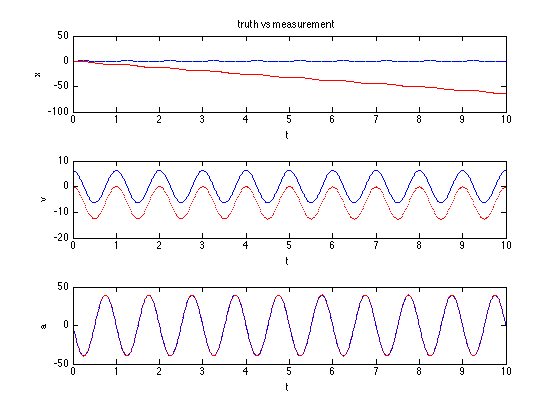
\includegraphics[width=\textwidth]{figures/foo1-uncorr.png}
\caption{Simple integration fails if the initial conditions are wrong, even if only a little, due to integrator drift.}
\label{fig:fail1}
\end{figure}

All is not lost, however.  We can fix this particular problem by also estimating the initial conditions and correcting for them.  If those are included in our measurement equations:
\begin{equation}
\ddot{x}^*[n] = \ddot{x}_n[n]
\end{equation}
\begin{equation}
\dot{x}^*[n] = \sum_{i=1}^n T_a \ddot{x}^*[i] + \dot{x}^*[0]
\end{equation}
\begin{equation}
x^*[n] = \sum_{i=1}^n T_a \dot{x}^*[i] + x^*[0]
\end{equation}

We have not yet made use of our position measurements, $x_m[m]$. Let us interpolate $x^*[n]$ to get $x^*[m]$ and then compute the error in the position estimate, which we hope is small:
\begin{equation}
x_m[m] - x^*[m] \approx 0 \mbox{(hopefully)}
\end{equation}
\begin{equation}
x_m[m] - x^*[0] - \dot{x}^*[0] m T_x - \sum \sum T_m^2 \ddot{x}_m[j] \approx 0
\end{equation}
We can solve numerically for $x^*[0]$ and $\dot{x}^*[0]$ that give the smallest error, for example, using a pseudo-inverse to make this as zeroish as we can, in a least-squares sense:
\begin{equation}
\begin{pmatrix}
1 & T_x \\
1 & 2T_x \\
\vdots & \vdots\\
1 & mT_x
\end{pmatrix}
\begin{pmatrix}
x^*[0]\\
\dot{x}^*[0]
\end{pmatrix}
= 
\begin{pmatrix}
x_m[1]-\sum_1^1\sum T_M^2 \ddot{x}_m[j] \\
x_m[2]-\sum_1^2\sum T_M^2 \ddot{x}_m[j] \\
\vdots\\
x_m[m]-\sum_1^m\sum T_M^2 \ddot{x}_m[j] \\
\end{pmatrix}
\end{equation}
\begin{equation}
\mathbf{A} \vec{p} = \vec{e_x}
\end{equation}
\begin{equation}
\hat{p} = (\mathbf{A}^T \mathbf{A})^{-1} \mathbf{A}^T \vec{e_x}
\end{equation}

\begin{figure}
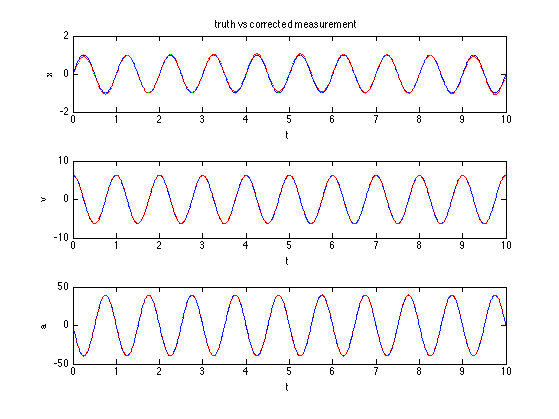
\includegraphics[width=\textwidth]{figures/foo1-corr.png}
\caption{Simple integration fails with corrections for initial conditions.}
\label{fig:corr1}
\end{figure}

This appears to work well enough, as shown in Figure~\ref{fig:corr1}. However, what if there are also offsets and gain errors in the sensors?  It turns out these can be accommodated with only slight modification.  We have two additional basis vectors on which to project our error, resulting in two extra numbers to solve for.  This should not be a problem so long as we have a lot of measurements, which we do:
\begin{equation}
\begin{pmatrix}
1 & T_x & T_x^2 & \tilde{x}[1]    \\
1 & 2T_x & 4T_x^2 & \tilde{x}[2] \\
\vdots & \vdots & \vdots & \vdots \\
1 & mT_x & m^2 T_x^2 & \tilde{x}[m] 
\end{pmatrix}
\begin{pmatrix}
x^*[0]\\
\dot{x}^*[0] \\
\ddot{x}^*[0] \\
K_x
\end{pmatrix}
= 
\begin{pmatrix}
e_x[1]\\
e_x[2]\\
\vdots \\
e_x[m]
\end{pmatrix}
\end{equation}
where $\tilde{x}$ here represents the naive double integral (sum) of $a_m$ and $K_x$ and $\ddot{x}^*[0]$ represent the gain and offset error, respectively, in the accelerometer.  It is easy enough to take a pseudo-inverse as before. 

This simple example illustrates the use of measurements to correct our estimate of the states and initial conditions.  However, there are other wrinkles we will have to deal with for the skydiving sensor problem, based on rotation of a sensor fixed to the body. 

\subsection{What if the sensor is fixed to the body?}
\label{sec:projectile}
To address the case of a sensor with axes fixed to the body, consider the case of an artillery projectile moving in two dimensions, without drag or spin.  The equations of motion are given by \cite{Galileo:1638, Newton:1687}:
\begin{equation}
y = \frac{1}{2}gt^2 + v_0 t + y_0
\end{equation}
\begin{equation}
x = u_0 t + x_0
\end{equation}
\begin{equation}
v = \frac{dy}{dt} = gt + v_0
\end{equation}
\begin{equation}
u = \frac{dx}{dt} = u_0
\end{equation}
\begin{equation}
a_y = \frac{d^2y}{dt^2} = g
\end{equation}
\begin{equation}
a_x = \frac{d^2x}{dt^2} = 0
\end{equation}
where $g=\SI{-9.81}{\meter\per\second\squared}$ \cite{Newton:1687}, positive $y$ is up and positive $x$ is right.  For the plots that follow below, we use initial conditions $x_0=\SI{0}{\meter}$, $y_0=\SI{0}{\meter}$, $u_0=\SI{50}{\meter\per\second}$, and $v_0=\SI{50}{\meter\per\second}$.  

The angle of the projectile with respect to horizontal, as might be seen by an angle-sensing magnetometer on the projectile, is:
\begin{equation}
\theta = \arctan{\frac{v}{u}}
\end{equation}
Also, using the chain rule, we can obtain the derivative of $\theta$, or the angular velocity that might be seen by a rate gyro on the projectile:
\begin{equation}
\omega = \frac{-v}{u^2+v^2}a_x + \frac{u}{u^2+v^2}a_y
\end{equation}
The accelerations sensed by a linear accelerometer fixed to the projectile will be in axes fixed to the body of the projectile:
\begin{equation}
\begin{pmatrix} a_t \\ a_n \end{pmatrix}
=
\begin{pmatrix}
\cos{\theta} & \sin{\theta} \\
-\sin{\theta} & \cos{\theta}
\end{pmatrix}
\begin{pmatrix} a_x \\ a_y \end{pmatrix}
\end{equation}
\begin{equation}
\vec{a}' = \mathbf{R}(\theta) \vec{a}
\end{equation}

As before, let us construct measurements of the state in which we sample the accelerometers and gyroscopes at \SI{50}{\hertz}, magnetometers at \SI{10}{\hertz}, and GPS positions at \SI{4}{\hertz}.  This is shown in figure~\ref{fig:projectile}.
\begin{figure}
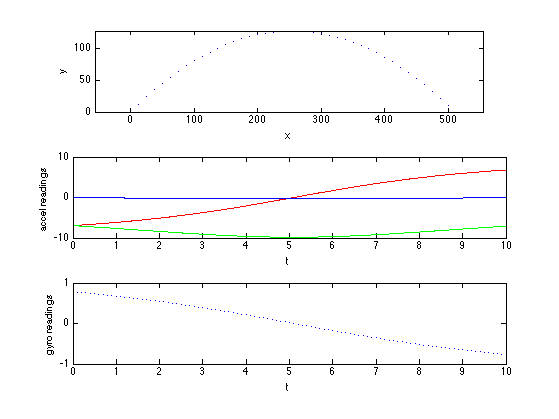
\includegraphics[width=\textwidth]{figures/foo2-raw.png}
\caption{Body-fixed sensor measurements for artillery projectile of section~\ref{sec:projectile}.}
\label{fig:projectile}
\end{figure}

We integrate this by working first with $\omega$ to obtain $\theta$, then using the inverse rotation operator $\mathbf{R}^{-1}(\theta) = \mathbf{R}(-\theta)$ to rotate the tangential and normal acceleration before integrating.  As before, we correct for initial conditions by finding the error in position estimates and projecting it onto basis vectors for constant, $t$, etc.  The results are shown in figure~\ref{fig:projectile-corr}.
\begin{figure}
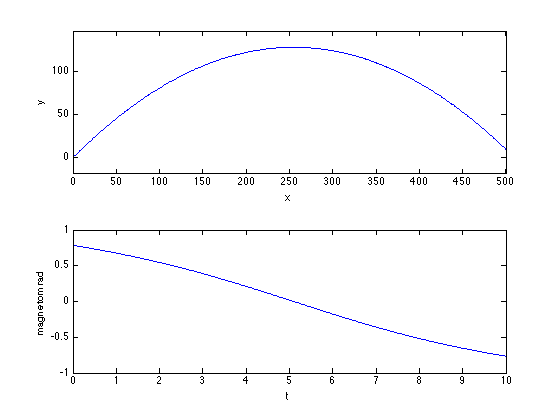
\includegraphics[width=\textwidth]{figures/foo2-corr.png}
\caption{Fused estimates of position for projectile problem, formed by estimating angle via integration, correcting angular position, transforming acceleration, integrating twice, and correcting position.}
\label{fig:projectile-corr}
\end{figure}




\section{Real data}
\subsection{Dealing with GPS coordinates}
\subsection{Rotations in 3D}
\subsection{Interpolation issues}

\section{Conclusions}

% AMS style references
\bibliographystyle{amsplain}
\bibliography{references/skydiving-kalman}
\end{document}
